\chapter{Perceptually Important Points}
\label{chap:pip}

Para atingir o primeiro objetivo -- proposto na seção \ref{sec:objetivos} --, escolheu-se o algoritmo \textit{Perceptually Important Points}, pois se mostrou conceitualmente simples em relação aos outros métodos apresentados no capítulo anterior, além de favorecer uma forma eficaz na redução de dimensionalidade de séries temporais.

\section{Ideia do algoritmo}
A primeira proposta formal do processo de identificação de \textit{Perceptually Important Points} foi introduzida por~\cite{firstpip} em uma análise técnica de padrões para aplicações financeiras, com ideias parecidas utilizadas em trabalhos independentes de~\cite{perng2000} e ~\cite{fink2003}. Entretanto, não é conhecida a utilização dessa técnica para o auxílio da representação de séries temporais de datacenters.

O algoritmo expressa um método para se definir que pontos são de fato imprescindíveis e que devem ser considerados para que a plotagem do gráfico preserve sua forma original para um observador humano.


Para ilustrar a ideia do algoritmo, vamos utilizar como série base, uma amostra de 50 pontos de uma função seno multiplicada por um fator aleatório entre 0 e 5 -- para incluir algum ruído nos dados, ilustrada na figura \ref{fig:original}.

Para podermos identificar os pontos mais importantes de uma série, é preciso considerá-la como um todo. Alguns pontos podem ser importantes em um período, mas completamente descartáveis quando se considera toda a sua história. Por essa razão, faz parte da inicialização do algoritmo incluir o primeiro e último pontos da série original, veja figura \ref{fig:inicializacao-pip}. 

Em sua primeira iteração, calculamos a distância de todos os pontos no intervalo com relação aos primeiros pontos escolhidos na inicialização. O ponto que possuir maior distância dos dois primeiros será o próximo ponto a ser promovido a PIP.

Após a primeira iteração, processamos todas as distâncias, agora para os dois intervalos implícitos pelos 3 pontos já escolhidos. Escolhemos nessa iteração o ponto que possui a maior distância desses intervalos e o promovemos a PIP. O processo se repete até que todos os pontos sejam escolhidos e estejam devidamente ordenados. 

Outros procedimentos e condições de parada podem ser definidos, como por exemplo, um valor fixo para o número de pontos a serem escolhidos, ou a atribuição de um erro tolerável. Tais condições serão discutidas ainda neste capítulo na seção \ref{sec:pseudo-algoritmo}.

\begin{figure}[htb!]
  \begin{center}
    \subfloat[Série original com 50 pontos.]{\label{fig:original}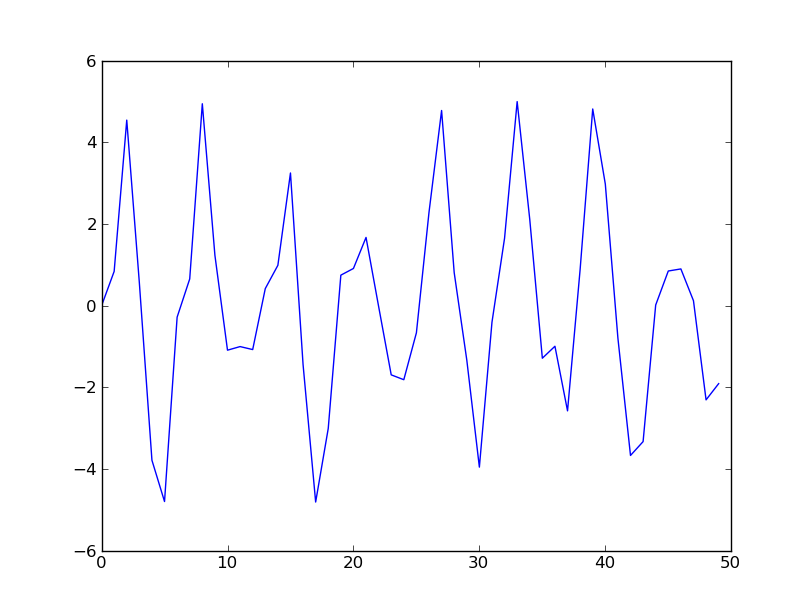
\includegraphics[width=0.5\textwidth]{original}}
    \\
    \subfloat[Inicialização.]{\label{fig:inicializacao-pip}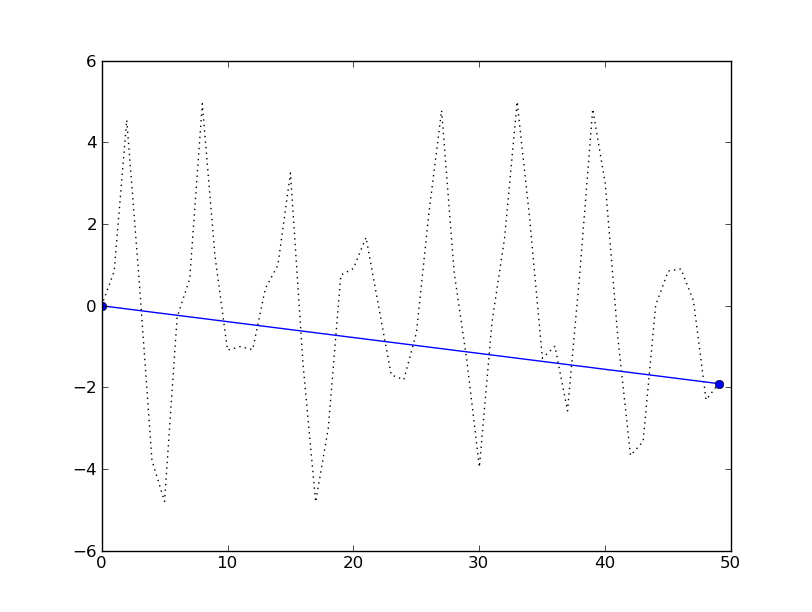
\includegraphics[width=0.4\textwidth]{pip2}}
    \subfloat[5 PIPs.]{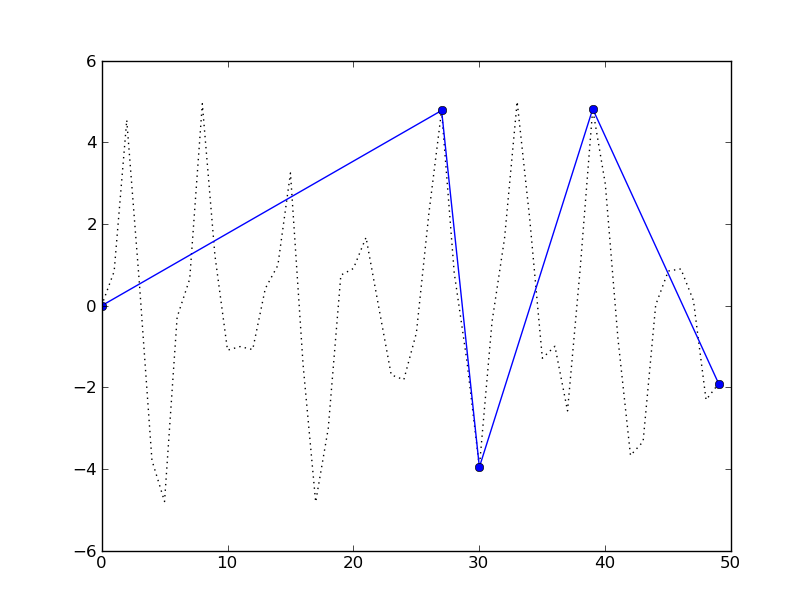
\includegraphics[width=0.4\textwidth]{pip5}}
    \\
    \subfloat[10 PIPs.]{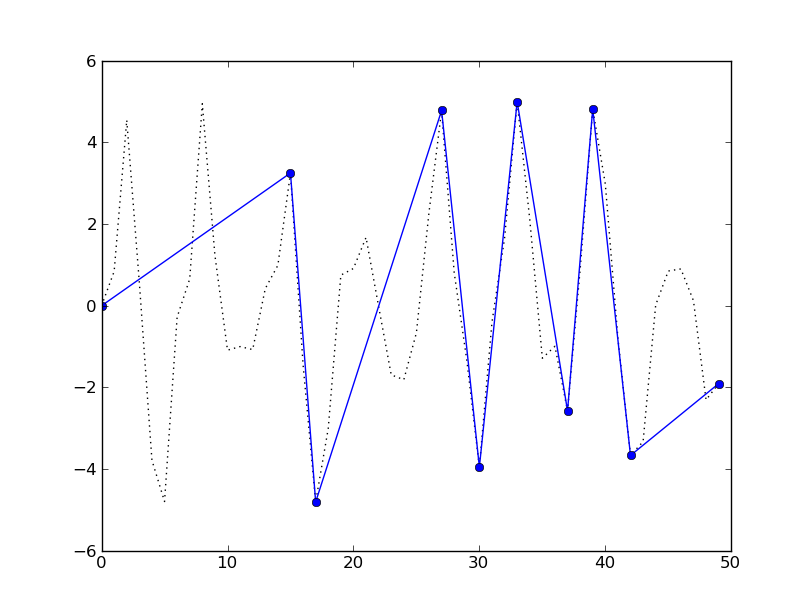
\includegraphics[width=0.4\textwidth]{pip10}}
    \subfloat[20 PIPs.]{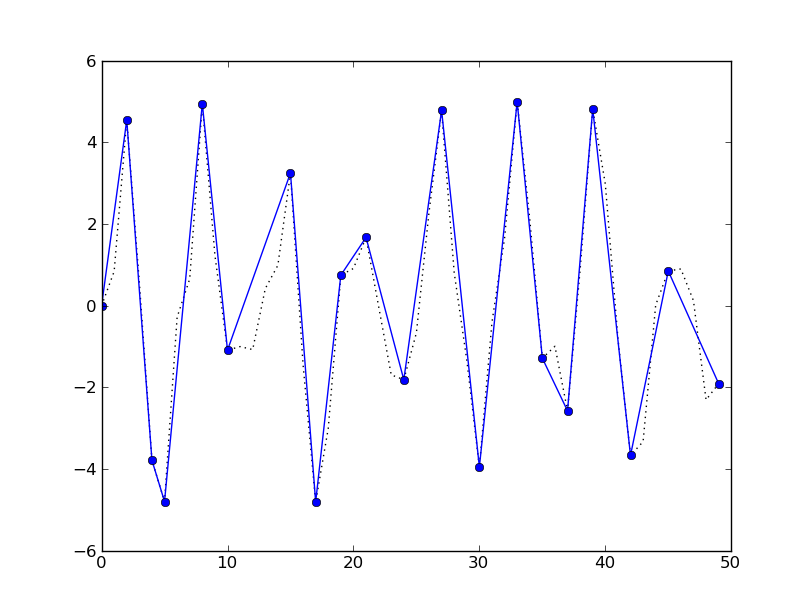
\includegraphics[width=0.4\textwidth]{pip20}}
    \centering
    \caption{Evolução do algoritmo PIP}
    \label{fig:evolucao}
  \end{center}
\end{figure}
\pagebreak

Na figura \ref{fig:evolucao}, conseguimos representar com 20 dos 50 pontos originais (descarte de 60 \% dos dados originais) a série com boa precisão visual, quase se confundindo com a série original para um observador humano. Compressões ainda melhores podem ser alcançadas dependendo da forma geral da série considerada. No apêndice \ref{chap:aproximacao}, pode-se visualizar a representação de uma série original de um mês de dados, com 8582 pontos sendo reduzida para apenas 300 pontos (descarte de aproximadamente 99.97\% dos pontos originais), com uma boa aproximação visual.


\section{Cálculo de distâncias}
Em~\cite{Fu2008} são apresentados testes comparativos com três abordagens diferentes para o cálculo de distâncias entre pontos: distância vertical, distância perpendicular e distância euclidiana. Constatou-se que a distância vertical apresentava os melhores resultados, e portanto, foi a escolhida para este trabalho.

Na figura \ref{fig:vertical-distance} podemos capturar a ideia por trás do cálculo da distância vertical. Os pontos $p1$ e $p2$ representam PIPs previamente escolhidos e o ponto $P3$ um candidato a ser promovido a PIP.
Este método incorpora a intuição de que flutuações verticais são mais importantes para um observador humano.

Em termos práticos, é utilizada a equação \ref{eq:vd} para calcular a distância entre pontos no algoritmo. Podem ser utilizadas técnicas de geometria analítica para se chegar na equação \ref{eq:vd} para o cálculo de distância vertical.

\begin{equation}
\label{eq:vd}
VD(p_{3}, p_{c}) = \mid y_{3} - y_{c} \mid = \mid \Bigg( y_{1} + (y_{2} - y_{1})\bigg(\frac{ x_{3} - x_{1} }{x_{2} - x_{1}}\bigg) \Bigg) - y_{3} \mid
\end{equation}

\begin{figure}[h!]
  \begin{center}
    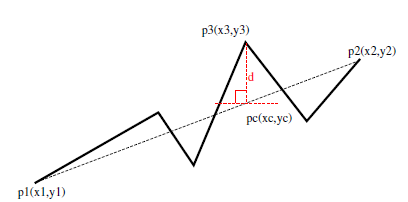
\includegraphics[width=0.6\textwidth]{vertical_distance}
    \centering
    \caption{Distância vertical.}
  \label{fig:vertical-distance}
  \end{center}
\end{figure}

\section{Pseudo-algoritmo}
\label{sec:pseudo-algoritmo}
Pseudo-algoritmos tem seu papel fundamental em estabelecer as macro operações que devem ser realizadas para a resolução de um problema, independente de linguagem de programação, facilitando o entendimento do leitor e o endereçamento de algumas observações sobre o método.

A entrada do algoritmo esperada é uma lista de pontos da série temporal original. Sua saída é um subconjunto desses pontos, que supostamente deveriam ser os mais significativos para um observador humano.

Nas linha 1 e 2 inicializamos a lista de PIPs com o primeiro e último pontos da série. O bloco delimitado pelas linhas 3 a 6 itera sobre os pontos de entrada procurando pelo próximo ponto mais significativo a cada iteração. É importante perceber que a cada iteração são promovidos a PIP apenas um ponto, pois devemos considerar séries temporais por inteiro para não cair em ótimos locais.

\begin{algorithm}[h!]
  \caption{Pseudo-algoritmo Perceptually Important Points}
  \label{alg:PIP1}
  \begin{algorithmic}[1]
  \REQUIRE Lista de pontos da série original $INPUT[1..n]$ ordenada 
  \ENSURE Lista de PIPs $PIP[1..n]$
  \STATE $PIP[1] \Leftarrow INPUT[1]$
  \STATE $PIP[2] \Leftarrow INPUT[n]$
  \REPEAT
    \STATE Selecionar ponto $P-MAX$ de $INPUT$ com maior distância a pontos adjacentes da lista de PIPs. 
    \STATE Inserir $P-MAX$ em $PIP$
  \UNTIL {tenham sido escolhidos n pontos de $INPUT[1..n]$}
  \RETURN $PIP$
  \end{algorithmic}
\end{algorithm}

O pseudo-algoritmo \ref{alg:PIP1} retorna sempre a mesma lista com todos os pontos originais, ainda que a ordem com que sejam escolhidos os pontos revele a importância de cada ponto, a resposta é sempre a mesma, a série original.
Pequenos ajustes podem ser considerados para deixar o algoritmo mais útil em termos práticos. Um deles é definir uma condição de parada para retornar apenas os $k <= n$ pontos mais importantes, exemplificado pelo pseudo-algoritmo \ref{alg:PIP2}.

\begin{algorithm}[h!]
  \caption{Pseudo-algoritmo Perceptually Important Points 2}
  \label{alg:PIP2}
  \begin{algorithmic}[1]
  \REQUIRE Lista de pontos da série original $INPUT[1..n]$ ordenada
  \REQUIRE $k$ pontos a serem escolhidos
  \ENSURE Lista de PIPs $PIP[1..k]$
  \STATE $PIP[1] \Leftarrow INPUT[1]$
  \STATE $PIP[2] \Leftarrow INPUT[n]$
  \REPEAT
    \STATE Selecionar ponto $P-MAX$ de $INPUT$ com maior distância a pontos adjacentes da lista de PIPs. 
    \STATE Inserir $P-MAX$ em $PIP$
  \UNTIL {tenham sido escolhidos $k$ pontos de $INPUT[1..n]$}
  \RETURN $PIP$
  \end{algorithmic}
\end{algorithm}

\subsection{Análise de Complexidade}
Pelo pseudo-algoritmo \ref{alg:PIP1}, podemos observar que as linhas 1, 2 e 7 são executadas em tempo constante. Para fins de análise de complexidade podemos portanto, eliminá-las do cálculo. O bloco delimitado pelas linhas 3 a 6 representam o maior tempo de computação e por isso devemos analisá-lo com mais cuidado.

Na linha 4 são selecionados pontos com maior distância a pontos adjancentes da lista atual de PIPs. Como a cada iteração são promovidos a PIP apenas um ponto e na inicialização já escolhemos dois destes -- primeiro e último da série original -- são selecionados a cada iteração, $(n - 2, n - 3, n - 4, ..., 3, 2, 1)$ pontos para comparação de distâncias. 

Inserir o ponto promovido a PIP na iteração corrente, linha 5, pode ser considerada constante, dependendo da estrutura de dados que se utiliza\footnote{Para a implementação, explicada com mais detalhes no próximo capítulo, as inserções são na verdade $O(log_{32} n)$, pois foi preferida a utilização de \textit{hashsets}, mas que na prática pode ser considerado constante.}.

Sendo assim, a complexidade do algoritmo é dada pelo número de cálculos de distâncias que fazemos no total, e pode ser calculado como:

\[
 \sum_{i=1}^{n - 2} i = \frac{n^2 - 3n + 2}{2}
\]

Deste modo, a complexidade do algoritmo é dada por $O(n^2)$. Já para o pseudo-algoritmo \ref{alg:PIP2}, o mesmo raciocínio pode ser traçado e sua complexidade de tempo é $O(nk)$.

\section{Cálculo de erro}
\label{sec:calculo-erro}
Como destacado na seção \ref{sec:pseudo-algoritmo}, pequenas variantes do pseudo-algoritmo apresentado podem ser implementadas para solucionar algumas dificuldades. Para o pseudo-algoritmo 2 é preciso escolher como entrada o número $k$ de pontos que se deseja resgatar da série original. Normalmente a escolha desse valor não gera bons resultados sem o conhecimento \textit{a priori} da série original.


\begin{figure}[htb!]
  \begin{center}
    \subfloat[Série com 100 pontos, variância muito alta]{\label{fig:alta-variancia}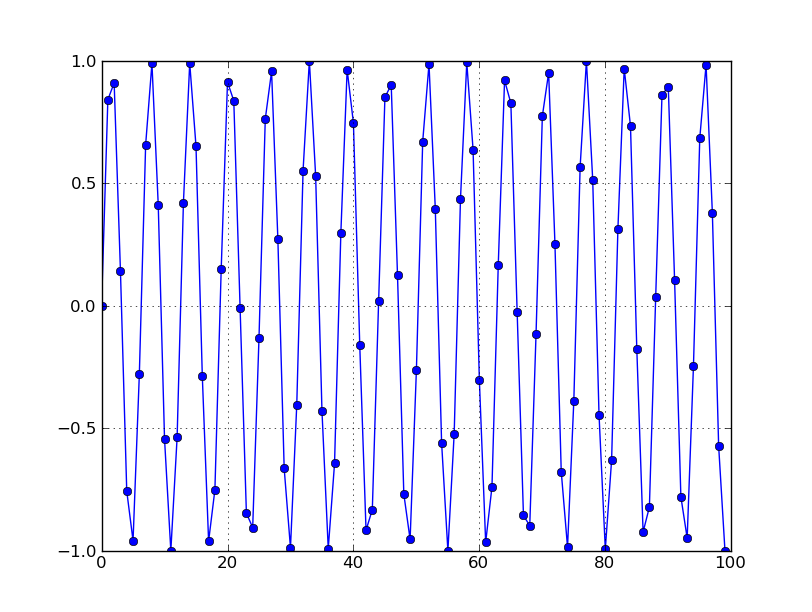
\includegraphics[width=0.4\textwidth]{random-serie}}
    \subfloat[Série com 100 pontos, baixa variância]{\label{fig:baixa-variancia}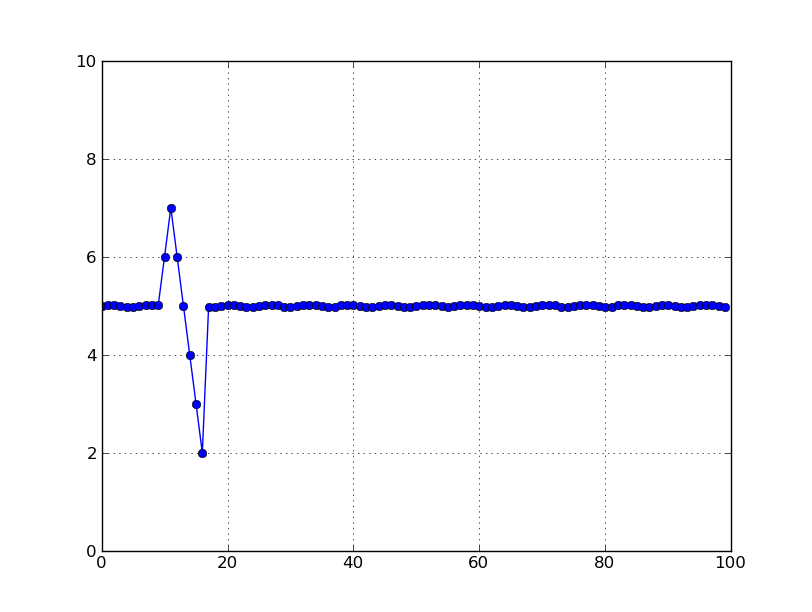
\includegraphics[width=0.4\textwidth]{nice-serie}}
    \centering
    \caption[Variância influencia número de PIPs]{Séries com o mesmo número de pontos podem necessitar de valores bem distintos de PIPs para serem representadas visualmente de modo satisfatório.}
    \label{fig:k-n}
  \end{center}
\end{figure}

Em geral, o valor de $k$ que representa razoavelmente bem\footnote{Como razoavelmente bem, busca-se o conceito subjetivo de similaridade entre duas séries temporais.} a série original não depende do valor de $n$. Para ilustrar tal afirmação, podemos visualizar a figura \ref{fig:k-n}. Na série da figura \ref{fig:alta-variancia}, um número maior de pontos são necessários para representá-la quando comparamos com a figura \ref{fig:baixa-variancia}, uma série mais bem comportada; ainda que as duas possuam a mesma quantidade de pontos no total, no caso 100.

\begin{algorithm}[h!]
  \caption{Pseudo-algoritmo Perceptually Important Points 3}
  \label{alg:PIP3}
  \begin{algorithmic}[1]
  \REQUIRE Lista de pontos da série original $INPUT[1..n]$ ordenada
  \REQUIRE Limite máximo $m$ de pontos a serem escolhidos
  \REQUIRE Erro $\epsilon$ aceitável
  \ENSURE Lista de PIPs $PIP[1..s]$, com $ s <= m$
  \STATE $PIP[1] \Leftarrow INPUT[1]$
  \STATE $PIP[2] \Leftarrow INPUT[n]$
  \REPEAT
    \STATE Selecionar ponto $P-MAX$ de $INPUT$ com maior distância a pontos adjacentes da lista de PIPs. 
    \STATE Inserir $P-MAX$ em $PIP$
  \UNTIL {$m$ pontos de $INPUT[1..n]$ já foram escolhidos ou tenha sido alcançada uma diferença menor que $\epsilon$} 
  \RETURN $PIP$
  \end{algorithmic}
\end{algorithm}

Sendo assim, como não é razoável que a entrada do valor de $k$ seja feita manualmente, é desejável um mecanismo automatizado de inferência sobre o menor valor de $k$ necessário para preservar a forma geral da série original. Para tanto, podem ser utilizadas diferença de mínimos quadrados a cada iteração do algoritmo, dando origem ao pseudo-algoritmo \ref{alg:PIP3}.

\section{Limitações do algoritmo}
\label{sec:limitacoes}
O algoritmo dá mais importância para as grandes flutuações em detrimento de variações mais suaves. O número mínimo de pontos necessários para representar razoavelmente bem uma série está diretamente ligado ao número de picos e vales que a série possui. Para séries com muitos picos e vales com alta amplitude, o algoritmo não consegue uma redução de dimensionalidade significativa.

